\documentclass[a4paper,10pt]{article}
\usepackage[utf8]{inputenc}
\usepackage[spanish]{babel}
\usepackage[affil-it]{authblk}
\usepackage{enumerate}
\usepackage{graphicx}
\usepackage{hyperref}
\usepackage{amsmath}
\usepackage{amssymb}
\usepackage{cancel}
\usepackage[usenames, dvipsnames]{color}
\usepackage{tikz}
\usepackage[labelfont=bf]{caption}
\usepackage{subcaption} %Multiple images
\usepackage{multicol} % Multiple columns
\usepackage{float}
\usepackage{cleveref}
 \usepackage{relsize} % bigger math symbols
\usepackage[margin=1.4in]{geometry}
\usepackage[titletoc,toc,title]{appendix}
\usepackage{enumitem}
\usepackage{etoolbox}
\usetikzlibrary{calc}
\numberwithin{equation}{section}

% Circled words
\newcommand{\circled}[2][]{%
  \tikz[baseline=(char.base)]{%
    \node[shape = circle, draw, inner sep = 1pt]
    (char) {\phantom{\ifblank{#1}{#2}{#1}}};%
    \node at (char.center) {\makebox[0pt][c]{#2}};}}
\robustify{\circled}

%Appendices in spanish
\renewcommand{\appendixname}{Ap\'endices}
\renewcommand{\appendixtocname}{Ap\'endices}
\renewcommand{\appendixpagename}{Ap\'endices}

%Zero delimiter
\newcommand{\zerodel}{.\kern-\nulldelimiterspace}

%Columns separation
\setlength{\columnsep}{1cm}

%Indentation
\setlength{\parindent}{0ex}

%Multiple References

\crefrangelabelformat{equation}{(#3#1#4--#5\crefstripprefix{#1}{#2}#6)}

\usepackage{xparse}

%Boxes

\newcommand*{\boxcolor}{blue}
\makeatletter
\renewcommand{\boxed}[1]{\textcolor{\boxcolor}{%
\tikz[baseline={([yshift=-1ex]current bounding box.center)}] \node [rectangle, minimum width=1ex,rounded corners,draw] {\normalcolor\m@th$\displaystyle#1$};}}
 \makeatother

%Constantes
\newcommand{\euler}{\mathrm{e}}
\newcommand{\im}{i}

%Lemas, teoremas, definiciones y pruebas
\newcommand{\definicion}{\textbf{Definición: }}
\newcommand{\lema}{\textbf{Lema: }}
\newcommand{\teorema}{\textbf{Teorema: }}
\newcommand{\prueba}{\textbf{Prueba: }}
\newcommand{\proposicion}{\textbf{Proposición: }}
\newcommand{\corolario}{\textbf{Corolario: }}

% Definición de las secciones y su numeración

\makeatletter
\def\@seccntformat#1{%
  \expandafter\ifx\csname c@#1\endcsname\c@section\else
  \csname the#1\endcsname\quad
  \fi}
\makeatother

%opening
\title{Mecánica Clásica Tarea \# 12}
\author{Favio Vázquez\thanks{Correo: favio.vazquezp@gmail.com}}\affil{Instituto de Ciencias Nucleares. Universidad Nacional Autónoma de México.}
\date{}

\begin{document}

\makeatletter
\def\@maketitle{%
  \newpage
  \null
  \vskip 2em%
  \begin{center}%
  \let \footnote \thanks
    {\Large\bfseries \@title \par}%
    \vskip 1.5em%
    {\normalsize
      \lineskip .5em%
      \begin{tabular}[t]{c}%
        \@author
      \end{tabular}\par}%
    \vskip 1em%
    {\normalsize \@date}%
  \end{center}%
  \par
  \vskip 1.5em}
\makeatother

\maketitle

\section{Problema 1}

Demuestre que entre los paréntesis de Poisson y los de Lagrange existe la relación 
de inversión

$$
\sum_{\alpha=1}^{2n} [u_\alpha,u_\beta]\{u_\alpha,u_\gamma\} = \delta_{\beta\gamma},
$$

donde $u_\alpha(q^1,\dots,q^n,p_1,\dots,p_n)$, $\alpha = 1, \dots, 2n$ y $(q,p)$ es un 
sistema canónico de coordenadas.

\vspace{.3cm}

\underline{Solución:} \vspace{.3cm}

Para demostrar esto utilizaremos la definición de cada uno de los paréntesis y 
las sustituiremos directamente. El paréntesis de Lagrange para las coordenadas 
canónicas $(q,p)$ y aplicados al problema en cuestión se escribe como

\begin{equation}
 [u_\alpha,u_\beta] = \sum_i^n \left( \frac{\partial q^i}{\partial u_\alpha}
 \frac{\partial p_i}{\partial u_\beta}- \frac{\partial q^i}{\partial u_\beta}
 \frac{\partial p_i}{\partial u_\alpha}\right),
\end{equation}

y el paréntesis de Poisson se escribe como 

\begin{equation}
 \{u_\alpha, u_\gamma\} = \sum_j^n \left( \frac{\partial u_\alpha}{\partial q^j}
 \frac{\partial u_\gamma}{\partial p_j} - \frac{\partial u_\alpha}{\partial p_j}
 \frac{\partial u_\gamma}{\partial q^j} \right).
\end{equation}

Tenemos entonces que 

\begin{align*}
\sum_{\alpha=1}^{2n} [u_\alpha,u_\beta]\{u_\alpha,u_\gamma\} &= 
\sum_{\alpha=1}^{2n} \left[\sum_i^n \left( \frac{\partial q^i}{\partial u_\alpha}
 \frac{\partial p_i}{\partial u_\beta}- \frac{\partial q^i}{\partial u_\beta}
 \frac{\partial p_i}{\partial u_\alpha}\right) \right] \left[ \sum_j^n \left( \frac{\partial u_\alpha}{\partial q^j}
 \frac{\partial u_\gamma}{\partial p_j} - \frac{\partial u_\alpha}{\partial p_j}
 \frac{\partial u_\gamma}{\partial q^j} \right)\right] \\
 &= \sum_{\alpha=1}^{2n} \sum_i^n \sum_j^n \left( \frac{\partial q^i}{\partial u_\alpha}
 \frac{\partial p_i}{\partial u_\beta}- \frac{\partial q^i}{\partial u_\beta}
 \frac{\partial p_i}{\partial u_\alpha}\right)\left( \frac{\partial u_\alpha}{\partial q^j}
 \frac{\partial u_\gamma}{\partial p_j} - \frac{\partial u_\alpha}{\partial p_j}
 \frac{\partial u_\gamma}{\partial q^j} \right) \\
 &= \sum_{\alpha=1}^{2n} \sum_i^n \sum_j^n \left[\frac{\partial q^i}{\partial u_\alpha}
 \frac{\partial p_i}{\partial u_\beta} \frac{\partial u_\alpha}{\partial q^j}
 \frac{\partial u_\gamma}{\partial p_j} - \frac{\partial q^i}{\partial u_\alpha}
 \frac{\partial p_i}{\partial u_\beta}\frac{\partial u_\alpha}{\partial p_j}
 \frac{\partial u_\gamma}{\partial q^j}  \right\zerodel \\
 &\left\zerodel- \frac{\partial q^i}{\partial u_\beta}\frac{\partial p_i}{\partial u_\alpha}
 \frac{\partial u_\alpha}{\partial q^j}\frac{\partial u_\gamma}{\partial p_j} + 
 \frac{\partial q^i}{\partial u_\beta}\frac{\partial p_i}{\partial u_\alpha}
 \frac{\partial u_\alpha}{\partial p_j}\frac{\partial u_\gamma}{\partial q^j}\right].
\end{align*}

Ahora evaluando estos términos vemos que 

\begin{align}
 \sum_{\alpha=1}^{2n} \frac{\partial q^i}{\partial u_\alpha}
 \frac{\partial u_\alpha}{\partial q^j} = \delta^i_j, \\
  \sum_{\alpha=1}^{2n} \frac{\partial q^i}{\partial u_\alpha}
 \frac{\partial u_\alpha}{\partial p_j} = 0, \\
  \sum_{\alpha=1}^{2n} \frac{\partial p_i}{\partial u_\alpha}
 \frac{\partial u_\alpha}{\partial q^j} = 0, \\
  \sum_{\alpha=1}^{2n} \frac{\partial p_i}{\partial u_\alpha}
 \frac{\partial u_\alpha}{\partial p_jj} = \delta^i_j.
\end{align}

Donde $\delta^i_j$ es la delta de Kronecker. Entonces tenemos que 

\begin{align}
\begin{split}
 \sum_{\alpha=1}^{2n} [u_\alpha,u_\beta]\{u_\alpha,u_\gamma\} &= \sum_i^n \sum_j^n
 \left( \frac{\partial p_i}{\partial u_\beta}\frac{\partial u_\gamma}{\partial p_j}\delta^i_j
 + \frac{\partial q^i}{\partial u_\beta}\frac{\partial u_\gamma}{\partial q^j}\delta^i_j\right) \\
 &= \sum_i^n \left( \frac{\partial p_i}{\partial u_\beta}\frac{\partial u_\gamma}{\partial p_i}
 + \frac{\partial q^i}{\partial u_\beta}\frac{\partial u_\gamma}{\partial q^i}\right).
\end{split}
\end{align}

Haciendo ahora la sumatoria en $i$ vemos que esta expresión debe ser igual a la 
delta de Kronecker para $\beta$ y $\gamma$, por lo tanto 

\begin{equation}
 \boxed{\sum_{\alpha=1}^{2n} [u_\alpha,u_\beta]\{u_\alpha,u_\gamma\} = \delta_{\beta\gamma}.}
\end{equation}

Que era lo que se pidió demostrar, con lo cual vemos que los paréntesis de Poisson y 
los paréntesis de Lagrange forman matrices inversas la una para la otra.

\section{Problema 2}

Demuestre por tres vías distintas que las transformaciones 

\begin{align*}
 q^1 &= \frac{\sqrt{2P_1}\sen{Q^1}+P_2}{\sqrt{m\omega}} \\
 q^2 &= \frac{\sqrt{2P_1}\cos{Q^1}+Q^2}{\sqrt{m\omega}} \\
 p_1 &= \frac{\sqrt{m\omega}(\sqrt{2P_1}\cos{Q^1 - Q^2})}{2} \\
 p_2 &= \frac{\sqrt{m\omega}(\sqrt{2P_1}\sen{Q^1 - P_2})}{2}, 
\end{align*}

y

\begin{align*}
 q^1 &= Q^1\cos{\lambda} + \frac{P_2\sen{\lambda}}{m\omega} \\
 q^2 &= Q^2\cos{\lambda} + \frac{P_1\sen{\lambda}}{m\omega}\\
 p_1 &= - m\omega Q^2\sen{\lambda} + P_1 \cos{\lambda}\\
 p_2 &= - m\omega Q^1\sen{\lambda} + P_2 \cos{\lambda},
\end{align*}

son canónicas.

\vspace{.3cm}

\underline{Solución:} \vspace{.3cm}

Comencemos con las primeras transformaciones canónicas. La primera prueba que haremos 
es con los paréntesis de Poisson, que debe cumplirse que 

\begin{align}
 \begin{split}
  \{q^1,q^2\} = 0, \\
  \{q^1,p_2\} = 0, \\
  \{q^1,p_1\} = 1, \\
  \{p_1,p_2\} = 0, \\
  \{q^2,p_1\} = 0, \\
  \{p_2, q^2\} = 1.
 \end{split}
\end{align}

Todas las demás se obtienen intercambiando las variables y usando la anti-simetría 
de los paréntesis de Poisson. Comencemos con las pruebas,

\begin{align*}
 \{q^1,q^2\} &= \frac{\partial q^1}{\partial Q^1}\frac{\partial q^2}{\partial P_1} - 
 \frac{\partial q^1}{\partial P_1}\frac{\partial q^2}{\partial Q^1} + 
 \cancelto{0}{\frac{\partial q^1}{\partial Q^2}}\frac{\partial q^2}{\partial P_2} -
 \frac{\partial q^1}{\partial P_2}\frac{\partial q^2}{\partial Q^2} \\
 &= \left(\frac{\cancel{\sqrt{2P_1}}\cos{Q^1}}{\sqrt{m\omega}} \right)
 \left(\frac{\cos{Q^1}}{\cancel{\sqrt{2P_1}}\sqrt{m\omega}} \right) \\
 &- \left(\frac{\sen{Q^1}}{\cancel{\sqrt{2P_1}}\sqrt{m\omega}} \right)
 \left(- \frac{\cancel{\sqrt{2P_1}}\sen{Q^1}}{\sqrt{m\omega}} \right) - 
 \left(\frac{1}{\sqrt{m\omega}}\right)\left(\frac{1}{\sqrt{m\omega}}\right) \\
 &= \frac{\cos^2{Q^1}}{m\omega} + \frac{\sen^2{Q^1}}{m\omega} - \frac{1}{m\omega} \\
 &= \frac{\cancelto{1}{\cos^2{Q^1} + \sen^2{Q^1}}}{m\omega} - \frac{1}{m\omega},
\end{align*}

\begin{equation}
 \therefore \{q^1,q^2\} = \frac{1}{m\omega} - \frac{1}{m\omega} = 0.
\end{equation}


\begin{align*}
 \{q^1,p_2\} &= \frac{\partial q^1}{\partial Q^1}\frac{\partial p_2}{\partial P_1} - 
 \frac{\partial q^1}{\partial P_1}\frac{\partial p_2}{\partial Q^1} + 
 \cancelto{0}{\frac{\partial q^1}{\partial Q^2}\frac{\partial p_2}{\partial P_2}} -
 \cancelto{0}{\frac{\partial q^1}{\partial P_2}\frac{\partial p_2}{\partial Q^2}} \\
 &= \left(\frac{\cancel{\sqrt{2P_1}}\cos{Q^1}}{\cancel{\sqrt{m\omega}}} \right)
 \left(\frac{\cancel{\sqrt{m\omega}}\sen{Q^1}}{2\cancel{\sqrt{2P_1}}} \right) - 
 \left(\frac{\sen{Q^1}}{\sqrt{2}\cancel{\sqrt{P_1}}\cancel{\sqrt{m\omega}}} \right)
 \left(\frac{\cancel{\sqrt{P_1}}\cancel{\sqrt{m\omega}}\cos{Q^1}}{\sqrt{2}}\right)
\end{align*}

\begin{equation}
 \therefore  \{q^1,p_2\} = \frac{\cos{Q^1}\sen{Q^1}}{2} - \frac{\cos{Q^1}\sen{Q^1}}{2} = 0
\end{equation}

\begin{align*}
 \{q^1,p_1\} &= \frac{\partial q^1}{\partial Q^1}\frac{\partial p_1}{\partial P_1} - 
 \frac{\partial q^1}{\partial P_1}\frac{\partial p_1}{\partial Q^1} + 
 \cancelto{0}{\frac{\partial q^1}{\partial Q^2}\frac{\partial p_1}{\partial P_2}} -
 \frac{\partial q^1}{\partial P_2}\frac{\partial p_1}{\partial Q^2} \\
 &= \left(\frac{\cancel{\sqrt{2P_1}}\cos{Q^1}}{\cancel{\sqrt{m\omega}}} \right)
 \left(\frac{\cancel{\sqrt{m\omega}} \cos{Q^1}}{2\cancel{\sqrt{2P_1}}}\right) \\
 &- \left(\frac{\sen{Q^1}}{\sqrt{2}\cancel{\sqrt{P_1}}\cancel{\sqrt{m\omega}}} \right)
 \left(\frac{\cancel{\sqrt{P_1}}\cancel{\sqrt{m\omega}}\sen{Q^1}}{\sqrt{2}} \right) -
 \left(\frac{1}{\cancel{\sqrt{m\omega}}} \right) \left(- \frac{\cancel{\sqrt{m\omega}}}{2} \right) \\ 
 &= \frac{\cos^2{Q^1}}{2} + \frac{\sen^2{Q^1}}{2} + \frac{1}{2} \\
 &= \frac{\cancelto{1}{\cos^2{Q^1} + \sen^2{Q^1}}}{2} + \frac{1}{2}
\end{align*}

\begin{equation}
 \therefore \{q^1,p_1\} = \frac{1}{2} + \frac{1}{2} = 1.
\end{equation}

\begin{align*}
  \{p_1,p_2\} &= \frac{\partial p_1}{\partial Q^1}\frac{\partial p_2}{\partial P_1} - 
 \frac{\partial p_1}{\partial P_1}\frac{\partial p_2}{\partial Q^1} + 
 \frac{\partial p_1}{\partial Q^2}\frac{\partial p_2}{\partial P_2} -
 \cancelto{0}{\frac{\partial p_1}{\partial P_2}\frac{\partial p_2}{\partial Q^2}} \\
 &= \left(-\frac{\cancel{\sqrt{P_1}}\sqrt{m\omega}\sen{Q^1}}{\sqrt{2}} \right)
 \left(\frac{\sqrt{m\omega}\sen{Q^1}}{2\sqrt{2}\cancel{\sqrt{P_1}}} \right) - 
 \left(\frac{\sqrt{m\omega}\cos{Q^1}}{2\sqrt{2}\cancel{\sqrt{P_1}}} \right) 
 \left(\frac{\cancel{\sqrt{P_1}}\sqrt{m\omega}\cos{Q^1}}{\sqrt{2}} \right) \\
 &- \left(-\frac{\sqrt{m\omega}}{2}\right)\left(-\frac{\sqrt{m\omega}}{2} \right) \\
 &= -\frac{m\omega \sen^2{Q^1}}{4} - \frac{m\omega \cos^2{Q^1}}{4} 
 + \frac{m\omega}{4}\\
 &= - \frac{m\omega}{4}(\cancelto{1}{\sen^2{Q^1} + \cos^2{Q^1}}) + \frac{m\omega}{4},
\end{align*}

\begin{equation}
 \therefore \{p_1,p_2\} = -  \frac{m\omega}{4} +  \frac{m\omega}{4} = 0.
\end{equation}

\begin{align*}
 \{q^2, p_1\} &= \frac{\partial q^2}{\partial Q^1}\frac{\partial p_1}{\partial P_1} - 
 \frac{\partial q^2}{\partial P_1}\frac{\partial p_1}{\partial Q^1} + 
 \cancelto{0}{\frac{\partial q^2}{\partial Q^2}\frac{\partial p_1}{\partial P_2}} -
 \cancelto{0}{\frac{\partial q^2}{\partial P_2}\frac{\partial p_1}{\partial Q^2}} \\
 &= \left(- \frac{\cancel{\sqrt{2P_1}}\sen{Q^1}}{\cancel{\sqrt{m\omega}}} \right)
 \left(\frac{\cancel{\sqrt{m\omega}}\cos{Q^1}}{2\cancel{\sqrt{2P_1}}} \right) - 
 \left(\frac{\cos{Q^1}}{\sqrt{2}\cancel{\sqrt{P_1}}\cancel{\sqrt{m\omega}}} \right)
 \left(- \frac{\cancel{\sqrt{P_1}}\cancel{\sqrt{m\omega}}\sen{Q^1}}{\sqrt{2}} \right)
\end{align*}

\begin{equation}
 \therefore \{q^2, p_1\} = - \frac{\sen{Q^1}\cos{Q^1}}{2} + \frac{\sen{Q^1}\cos{Q^1}}{2} = 0
\end{equation}

\begin{align*}
 \{q^2, p_2\} &= \frac{\partial q^2}{\partial Q^1}\frac{\partial p_2}{\partial P_1} - 
 \frac{\partial q^2}{\partial P_1}\frac{\partial p_2}{\partial Q^1} + 
 \frac{\partial q^2}{\partial Q^2}\frac{\partial p_2}{\partial P_2} -
 \cancelto{0}{\frac{\partial q^2}{\partial P_2}\frac{\partial p_2}{\partial Q^2}} \\
 &=  \left(- \frac{\cancel{\sqrt{2P_1}}\sen{Q^1}}{\cancel{\sqrt{m\omega}}} \right)
 \left(\frac{\cancel{\sqrt{m\omega}}\sen{Q^1}}{2\cancel{\sqrt{2P_1}}} \right) - 
 \left(\frac{\cos{Q^1}}{\sqrt{2}\cancel{\sqrt{P_1}}\cancel{\sqrt{m\omega}}} \right)
 \left(\frac{\sqrt{P_1}\sqrt{m\omega}\cos{Q^1}}{\sqrt{2}} \right) \\
 &+ \left(\frac{1}{\cancel{\sqrt{m\omega}}}\right)\left(- \frac{\cancel{\sqrt{m\omega}}}{2} \right) \\
 &= - \frac{\sen^2{Q^1}}{2} - \frac{\cos^2{Q^1}}{2} - \frac{1}{2} \\
 &= - \frac{1}{2}(\cancelto{1}{(\sen^2{Q^1} + \cos^2{Q^1})}) - \frac{1}{2},
\end{align*}

\begin{equation}
 \{p_2, q^2\} = - \{q^2, p_2\} = \frac{1}{2} + \frac{1}{2} = 1.
\end{equation}

Probemos ahora con los paréntesis de Lagrange, que se debe cumplir que

\begin{align}
 \begin{split}
  [q^1,q^2] = 0, \\
  [q^1,p_2] = 0, \\
  [q^1,p_1] = 1, \\
  [p_1,p_2] = 0, \\
  [q^2,p_1] = 0, \\
  [p_2, q^2] = 1.
 \end{split}
\end{align}

Pero la prueba para los paréntesis de Lagrange es trivial al saber que 

\begin{equation}
 \sum_k^{2n} \{q^k,p_i\}[q^k,p_j] = \delta_{ij},
\end{equation}

que fue el resultado al cual se llegó en el problema anterior. Con lo cual tenemos que,
utilizando los resultados que hemos obtenidos arriba

\begin{align}
 \begin{split}
  [q^1,q^2] = \{q^1,q^2\} = 0, \\
  [q^1,p_2] = \{q^1,p_2\} = 0, \\
  [q^1,p_1] = \{q^1, p_1\} = 1, \\
  [p_1,p_2] = \{p_1,p_2\} = 0, \\
  [q^2,p_1] = \{q^2,p_1\} = 0, \\
  [p_2, q^2] = \{p_2,q^2\} = 1.
 \end{split}
\end{align}

La última prueba será demostrar que la transformación canónica deja invariante 
a la forma simpléctica. Para hacer esto debido a la forma complicada de las ecuaciones 
haremos el cálculo más general, de donde debe cumplirse que 

\begin{equation}
 dp_1 \wedge dq^1 + dp_2 \wedge dq^2 = dP_1 \wedge dQ^1 + dP_2 \wedge dQ^2.
\end{equation}

Usaremos las diferenciales para validar que se cumple esta igualdad,

\begin{align*}
 \gamma &= dp_1 \wedge dq^1 + dp_2 \wedge dq^2 \\
 &= \left(\frac{\partial p_1}{\partial Q^1}dQ^1 + \frac{\partial p_1}{\partial P_1}dP_1 + 
 \frac{\partial p_1}{\partial Q^2}dQ^2 + \frac{\partial p_1}{\partial P_2}dP_2 \right) 
 \wedge \left(\frac{\partial q^1}{\partial Q^1}dQ^1 + \frac{\partial q^1}{\partial P_1}dP_1 + 
 \frac{\partial q^1}{\partial Q^2}dQ^2 + \frac{\partial q^1}{\partial P_2}dP_2 \right) \\
 &+ \left(\frac{\partial p_2}{\partial Q^1}dQ^1 + \frac{\partial p_2}{\partial P_1}dP_1 + 
 \frac{\partial p_2}{\partial Q^2}dQ^2 + \frac{\partial p_2}{\partial P_2}dP_2 \right) 
 \wedge \left(\frac{\partial q^2}{\partial Q^1}dQ^1 + \frac{\partial q^2}{\partial P_1}dP_1 + 
 \frac{\partial q^2}{\partial Q^2}dQ^2 + \frac{\partial q^2}{\partial P_2}dP_2 \right) \\
 &= \frac{\partial p_1}{\partial Q^1}\frac{\partial q^1}{\partial Q^1}dQ^1 \wedge dQ^1 + 
 \frac{\partial p_1}{\partial Q^1}\frac{\partial q^1}{\partial P_1}dQ^1 \wedge dP_1 + 
 \cancelto{0}{\frac{\partial p_1}{\partial Q^1}\frac{\partial q^1}{\partial Q^2}}dQ^1 \wedge dQ^2 + 
 \frac{\partial p_1}{\partial Q^1}\frac{\partial q^1}{\partial P_2}dQ^1 \wedge dP_2 \\
 &+ \frac{\partial p_1}{\partial P_1}\frac{\partial q^1}{\partial Q^1} dP_1 \wedge dQ^1 +
 \frac{\partial p_1}{\partial P_1}\frac{\partial q^1}{\partial P_1} dP_1 \wedge dP_1 + 
 \cancelto{0}{\frac{\partial p_1}{\partial P_1}\frac{\partial q^1}{\partial Q^2}} dP_1 \wedge dQ^2 + 
 \frac{\partial p_1}{\partial P_1}\frac{\partial q^1}{\partial P_2} dP_1 \wedge dP_2 \\
 &+  \frac{\partial p_1}{\partial Q^2}\frac{\partial q^1}{\partial Q^1} dQ^2 \wedge dQ^1 
 + \frac{\partial p_1}{\partial Q^2}\frac{\partial q^1}{\partial P_1} dQ^2 \wedge dP_1 + 
 \cancelto{0}{\frac{\partial p_1}{\partial Q^2}\frac{\partial q^1}{\partial Q^2}} dQ^2 \wedge dQ^2 + 
 \frac{\partial p_1}{\partial Q^2}\frac{\partial q^1}{\partial P_2} dQ^2 \wedge dP_2 \\
 &+  \cancelto{0}{\frac{\partial p_1}{\partial P_2}\frac{\partial q^1}{\partial Q^1}} dP_2 \wedge dQ^1
 + \cancelto{0}{\frac{\partial p_1}{\partial P_2}\frac{\partial q^1}{\partial P_1}} dP_2 \wedge dP_1 + 
 \cancelto{0}{\frac{\partial p_1}{\partial P_2}\frac{\partial q^1}{\partial Q^2}} dP_2 \wedge dQ^2 + 
 \cancelto{0}{\frac{\partial p_1}{\partial P_2}\frac{\partial q^1}{\partial P_2}} dP_2 \wedge dP_2 \\
 %
 &+ \frac{\partial p_2}{\partial Q^1}\frac{\partial q^2}{\partial Q^1}dQ^1 \wedge dQ^1 + 
 \frac{\partial p_2}{\partial Q^1}\frac{\partial q^2}{\partial P_1}dQ^1 \wedge dP_1 + 
 \frac{\partial p_2}{\partial Q^1}\frac{\partial q^2}{\partial Q^2}dQ^1 \wedge dQ^2 + 
 \cancelto{0}{\frac{\partial p_2}{\partial Q^1}\frac{\partial q^2}{\partial P_2}}dQ^1 \wedge dP_2 \\
 &+ \frac{\partial p_2}{\partial P_1}\frac{\partial q^2}{\partial Q^1} dP_1 \wedge dQ^1 +
 \frac{\partial p_2}{\partial P_1}\frac{\partial q^2}{\partial P_1} dP_1 \wedge dP_1 + 
 \frac{\partial p_2}{\partial P_1}\frac{\partial q^2}{\partial Q^2} dP_1 \wedge dQ^2 + 
 \cancelto{0}{\frac{\partial p_2}{\partial P_1}\frac{\partial q^2}{\partial P_2}} dP_1 \wedge dP_2 \\
 &+  \cancelto{0}{\frac{\partial p_2}{\partial Q^2}\frac{\partial q^2}{\partial Q^1}} dQ^2 \wedge dQ^1 
 + \cancelto{0}{\frac{\partial p_2}{\partial Q^2}\frac{\partial q^2}{\partial P_1}} dQ^2 \wedge dP_1 + 
 \cancelto{0}{\frac{\partial p_2}{\partial Q^2}\frac{\partial q^2}{\partial Q^2}} dQ^2 \wedge dQ^2 + 
 \cancelto{0}{\frac{\partial p_2}{\partial Q^2}\frac{\partial q^2}{\partial P_2}} dQ^2 \wedge dP_2 \\
 &+  \frac{\partial p_2}{\partial P_2}\frac{\partial q^2}{\partial Q^1} dP_2 \wedge dQ^1
 + \frac{\partial p_2}{\partial P_2}\frac{\partial q^2}{\partial P_1} dP_2 \wedge dP_1 + 
 \frac{\partial p_2}{\partial P_2}\frac{\partial q^2}{\partial Q^2} dP_2 \wedge dQ^2 + 
 \cancelto{0}{\frac{\partial p_2}{\partial P_2}\frac{\partial q^2}{\partial P_2}} dP_2 \wedge dP_2.
\end{align*}

Agrupando términos y utilizando la propiedad de antisimetría del producto exterior, 

\begin{align*}
 \gamma &= dQ^1 \wedge dQ^1 \cancelto{0}{\left(\frac{\partial p_1}{\partial Q^1}\frac{\partial q^1}{\partial Q^1} 
 + \frac{\partial p_2}{\partial Q^1}\frac{\partial q^2}{\partial Q^1}\right)} + 
 dQ^1 \wedge dQ^2 \cancelto{0}{\left(- \frac{\partial p_1}{\partial Q^2}\frac{\partial q^1}{\partial Q^1} 
 +  \frac{\partial p_2}{\partial Q^1}\frac{\partial q^2}{\partial Q^2}\right)} \\
 &+ dP_1 \wedge dQ^1 \cancelto{1}{\left(- \frac{\partial p_1}{\partial Q^1}\frac{\partial q^1}{\partial P_1}
 + \frac{\partial p_1}{\partial P_1}\frac{\partial q^1}{\partial Q^1} 
 - \frac{\partial p_2}{\partial Q^1}\frac{\partial q^2}{\partial P_1} 
 + \frac{\partial p_2}{\partial P_1}\frac{\partial q^2}{\partial Q^1}\right)} \\
 &+ dQ^2 \wedge dP^1 \cancelto{0}{\left(\frac{\partial p_1}{\partial Q^2}\frac{\partial q^1}{\partial P_1} - 
 \frac{\partial p_2}{\partial P_1}\frac{\partial q^2}{\partial Q^2} \right)}
 + dP_1 \wedge dP_1 \cancelto{0}{\left(\frac{\partial p_1}{\partial Q^1}\frac{\partial q^1}{\partial P_1}
 + \frac{\partial p_2}{\partial Q^1}\frac{\partial q^2}{\partial Q^1}\right)} \\
 &+ dP_1 \wedge dP_2 \cancelto{0}{\left(\frac{\partial p_1}{\partial Q^1}\frac{\partial q^1}{\partial P_2} 
 - \frac{\partial p_2}{\partial P_2}\frac{\partial q^2}{\partial Q^2}\right)}
 + dP_2 \wedge dQ^2 \cancelto{1}{\left(- \frac{\partial p_1}{\partial Q^2}\frac{\partial q^1}{\partial P_2}
 + \frac{\partial p_2}{\partial P_2}\frac{\partial q^2}{\partial Q^2} \right)}.
\end{align*}

Las cancelaciones e igualaciones a 1 las hemos hecho utilizando todas las derivadas 
que obtuvimos anteriormente, con lo cual tenemos que 

\begin{equation}
 \gamma = dP_1 \wedge dQ^1 + dP_2 \wedge dQ^2,
\end{equation}

y por lo tanto hemos encontrado la relación que esperábamos,

\begin{equation}
 \boxed{dp_1 \wedge dq^1 + dp_2 \wedge dq^2 = dP_1 \wedge dQ^1 + dP_2 \wedge dQ^2.}
\end{equation}

\vspace{.3cm}

Para las segundas transformaciones canónicas, comencemos igual la prueba utilizando 
los paréntesis de Poisson, que recordamos que debe cumplirse que 

\begin{align}
 \begin{split}
  \{q^1,q^2\} = 0, \\
  \{q^1,p_2\} = 0, \\
  \{q^1,p_1\} = 1, \\
  \{p_1,p_2\} = 0, \\
  \{q^2,p_1\} = 0, \\
  \{q^2,p_2\} = 1.
 \end{split}
\end{align}

Entonces, 

\begin{align*}
  \{q^1,q^2\} &= \frac{\partial q^1}{\partial Q^1}\frac{\partial q^2}{\partial P_1} - 
 \cancelto{0}{\frac{\partial q^1}{\partial P_1}\frac{\partial q^2}{\partial Q^1}} + 
 \cancelto{0}{\frac{\partial q^1}{\partial Q^2}\frac{\partial q^2}{\partial P_2}} -
 \frac{\partial q^1}{\partial P_2}\frac{\partial q^2}{\partial Q^2} \\
 &= (\cos{\lambda})\left(\frac{\sen{\lambda}}{m\omega}\right) - 
 \left(\frac{\sen{\lambda}}{m\omega}\right)(\cos{\lambda}) 
\end{align*}

\begin{equation}
 \therefore  \{q^1,q^2\} =  \frac{\cos{\lambda}\sen{\lambda}}{m\omega} -
 \frac{\cos{\lambda}\sen{\lambda}}{m\omega} =0.
\end{equation}

\begin{align*}
 \{q^1,p_2\} &= \cancelto{0}{\frac{\partial q^1}{\partial Q^1}\frac{\partial p_2}{\partial P_1}} - 
 \cancelto{0}{\frac{\partial q^1}{\partial P_1}\frac{\partial p_2}{\partial Q^1}} + 
 \cancelto{0}{\frac{\partial q^1}{\partial Q^2}\frac{\partial p_2}{\partial P_2}} -
 \cancelto{0}{\frac{\partial q^1}{\partial P_2}\frac{\partial p_2}{\partial Q^2}}
\end{align*}

\begin{equation}
 \therefore  \{q^1,p_2\} = 0.
\end{equation}


\begin{align*}
 \{q^1,p_1\} &= \frac{\partial q^1}{\partial Q^1}\frac{\partial p_1}{\partial P_1} - 
 \cancelto{0}{\frac{\partial q^1}{\partial P_1}\frac{\partial p_1}{\partial Q^1}} + 
 \cancelto{0}{\frac{\partial q^1}{\partial Q^2}\frac{\partial p_1}{\partial P_2}} -
 \frac{\partial q^1}{\partial P_2}\frac{\partial p_1}{\partial Q^2} \\
 &= (\cos{\lambda})(\cos{\lambda}) - \left(\frac{\sen{\lambda}}{\cancel{m\omega}}\right)
 (- \cancel{m\omega} \sen{\lambda})
\end{align*}

\begin{equation}
 \therefore \{q^1,p_1\} = \cos^2{\lambda} + \sen^2{\lambda} = 1.
\end{equation}

\begin{align*}
  \{p_1,p_2\} &= \cancelto{0}{\frac{\partial p_1}{\partial Q^1}\frac{\partial p_2}{\partial P_1}} - 
 \frac{\partial p_1}{\partial P_1}\frac{\partial p_2}{\partial Q^1} + 
 \frac{\partial p_1}{\partial Q^2}\frac{\partial p_2}{\partial P_2} -
 \cancelto{0}{\frac{\partial p_1}{\partial P_2}\frac{\partial p_2}{\partial Q^2}} \\
 &= - (\cos{\lambda})(- m\omega\sen{\lambda}) + (- m\omega\sen{\lambda})(\cos{\lambda}) 
\end{align*}

\begin{equation}
 \therefore \{p_1,p_2\} = m\omega\cos{\lambda}\sen{\lambda} - 
 m\omega\cos{\lambda}\sen{\lambda} = 0.
\end{equation}

\begin{align*}
 \{q^2, p_1\} &= \cancelto{0}{\frac{\partial q^2}{\partial Q^1}\frac{\partial p_1}{\partial P_1}} - 
 \cancelto{0}{\frac{\partial q^2}{\partial P_1}\frac{\partial p_1}{\partial Q^1}} + 
 \cancelto{0}{\frac{\partial q^2}{\partial Q^2}\frac{\partial p_1}{\partial P_2}} -
 \cancelto{0}{\frac{\partial q^2}{\partial P_2}\frac{\partial p_1}{\partial Q^2}} 
\end{align*}

\begin{equation}
 \therefore  \{q^2, p_1\} = 0.
\end{equation}

\begin{align*}
 \{q^2, p_2\} &= \cancelto{0}{\frac{\partial q^2}{\partial Q^1}\frac{\partial p_2}{\partial P_1}} - 
 \frac{\partial q^2}{\partial P_1}\frac{\partial p_2}{\partial Q^1} + 
 \frac{\partial q^2}{\partial Q^2}\frac{\partial p_2}{\partial P_2} -
 \cancelto{0}{\frac{\partial q^2}{\partial P_2}\frac{\partial p_2}{\partial Q^2}} \\
 &= -\left(\frac{\sen{\lambda}}{\cancel{m\omega}}\right)(-\cancel{m\omega}\sen{\lambda}) + 
 (\cos{\lambda})(\cos{\lambda}) 
\end{align*}

\begin{equation}
 \therefore = \{q^2, p_2\} = \sen^2{\lambda} + \cos^2{\lambda} = 1.
\end{equation}

Probemos ahora con los paréntesis de Lagrange, que se debe cumplir que

\begin{align}
 \begin{split}
  [q^1,q^2] = 0, \\
  [q^1,p_2] = 0, \\
  [q^1,p_1] = 1, \\
  [p_1,p_2] = 0, \\
  [q^2,p_1] = 0, \\
  [q^2, p_2] = 1.
 \end{split}
\end{align}

De nuevo, la prueba con los paréntesis de Lagrange es trivial al saber que 

\begin{equation}
 \sum_k^{2n} \{q^k,p_i\}[q^k,p_j] = \delta_{ij},
\end{equation}

que fue el resultado al cual se llegó en el problema anterior. Con lo cual tenemos que,
utilizando los resultados que hemos obtenidos arriba

\begin{align}
 \begin{split}
  [q^1,q^2] = \{q^1,q^2\} = 0, \\
  [q^1,p_2] = \{q^1,p_2\} = 0, \\
  [q^1,p_1] = \{q^1, p_1\} = 1, \\
  [p_1,p_2] = \{p_1,p_2\} = 0, \\
  [q^2,p_1] = \{q^2,p_1\} = 0, \\
  [q^2, p_2] = \{q^2,p_2\} = 1.
 \end{split}
\end{align}

La última prueba será demostrar que la transformación canónica deja invariante 
a la forma simpléctica. Para hacer esto calculemos las diferenciales, 

\begin{align}
 dq^1 = \cos{\lambda}dQ^1 + \frac{\sen{\lambda}}{m\omega}dP_2, \\ 
 dq^2 = \cos{\lambda}dQ^2 + \frac{\sen{\lambda}}{m\omega}dP_1, \\
 dp_1 = - m\omega\sen{\lambda} dQ^2 + \cos{\lambda}dP_1, \\
 dp_2 = - m\omega\sen{\lambda} dQ^1 + \cos{\lambda}dP_2.
\end{align}

Hagamos ahora los siguientes productos exteriores, 

\begin{align}
\begin{split}
 dp_1 \wedge dq^1 &= (- m\omega\sen{\lambda} dQ^2 + \cos{\lambda}dP_1) \wedge 
  \left(\cos{\lambda}dQ^1 + \frac{\sen{\lambda}}{m\omega}dP_2\right) \\
  &= - m\omega\sen{\lambda}\cos{\lambda} dQ^2 \wedge dQ^1  
  - \cancel{m\omega}\sen{\lambda}\frac{\sen{\lambda}}{\cancel{m\omega}}dQ^2 \wedge dP_2 \\
  &+ \cos{\lambda}\cos{\lambda}dP_1 \wedge dQ^1 + 
  \cos{\lambda}\frac{\sen{\lambda}}{m\omega} dP_1 \wedge dP_2 \\
  &= - m\omega\sen{\lambda}\cos{\lambda} dQ^2 \wedge dQ^1
  - \sen^2{\lambda}dQ^2 \wedge dP_2 \\ 
  &+ \cos^2{\lambda}dP_1 \wedge dQ^1 + \frac{1}{m\omega}\cos{\lambda}\sen{\lambda} dP_1 \wedge dP_2.
  \label{eq:2parte2productoext1}
\end{split}
\end{align}

\begin{align}
\begin{split}
 dp_2 \wedge dq^2 &= (- m\omega\sen{\lambda} dQ^1 + \cos{\lambda}dP_2) \wedge 
 \left(\cos{\lambda}dQ^2 + \frac{\sen{\lambda}}{m\omega}dP_1\right) \\
 &= - m\omega\sen{\lambda}\cos{\lambda} dQ^1 \wedge dQ^2  
  - \cancel{m\omega}\sen{\lambda}\frac{\sen{\lambda}}{\cancel{m\omega}}dQ^1 \wedge dP_1 \\
  &+ \cos{\lambda}\cos{\lambda}dP_2 \wedge dQ^2 + 
  \cos{\lambda}\frac{\sen{\lambda}}{m\omega} dP_2 \wedge dP_1 \\
  &= - m\omega\sen{\lambda}\cos{\lambda} dQ^1 \wedge dQ^2
  - \sen^2{\lambda}dQ^1 \wedge dP_1 \\ 
  &+ \cos^2{\lambda}dP_2 \wedge dQ^2 + \frac{1}{m\omega}\cos{\lambda}\sen{\lambda} dP_2 \wedge dP_1.
  \label{eq:2parte2productoext2}
\end{split}
\end{align}

Entonces si la transformación es canónica debe cumplirse que 

\begin{equation}
 dp_1 \wedge dq^1 + dp_2 \wedge dq^2 = dP_1 \wedge dQ^1 + dP_2 \wedge dQ^2,
\end{equation}

sumemos entonces \eqref{eq:2parte2productoext1} con \eqref{eq:2parte2productoext2} a ver 
si se cumple esta igualdad,

\begin{align*}
 dp_1 \wedge dq^1 + dp_2 \wedge dq^2 &= - m\omega\sen{\lambda}\cos{\lambda} dQ^2 \wedge dQ^1
  - \sen^2{\lambda}dQ^2 \wedge dP_2 \\ 
  &+ \cos^2{\lambda}dP_1 \wedge dQ^1 + \frac{1}{m\omega}\cos{\lambda}\sen{\lambda} dP_1 \wedge dP_2 \\ 
  &- m\omega\sen{\lambda}\cos{\lambda} dQ^1 \wedge dQ^2
  - \sen^2{\lambda}dQ^1 \wedge dP_1 \\
  &+ \cos^2{\lambda}dP_2 \wedge dQ^2 + \frac{1}{m\omega}\cos{\lambda}\sen{\lambda} dP_2 \wedge dP_1.
\end{align*}

Si usamos la propiedad anti-simétrica del producto exterior la ecuación anterior 
puede escribirse como 

\begin{align*}
 dp_1 \wedge dq^1 + dp_2 \wedge dq^2 &= - \cancel{m\omega\sen{\lambda}\cos{\lambda} dQ^2 \wedge dQ^1}
  + \sen^2{\lambda}dP_2 \wedge dQ^2 \\ 
  &+ \cos^2{\lambda}dP_1 \wedge dQ^1 + \cancel{\frac{1}{m\omega}\cos{\lambda}\sen{\lambda} dP_1 \wedge dP_2} \\ 
  &+ \cancel{m\omega\sen{\lambda}\cos{\lambda} dQ^2 \wedge dQ^1}
  + \sen^2{\lambda}dP_1 \wedge dQ^1 \\
  &+ \cos^2{\lambda}dP_2 \wedge dQ^2 - \cancel{\frac{1}{m\omega}\cos{\lambda}\sen{\lambda} dP_1 \wedge dP_2}.
\end{align*}

\begin{equation}
 dp_1 \wedge dq^1 + dp_2 \wedge dq^2 =  \cancelto{1}{(\sen^2{\lambda} + \cos^2{\lambda})}dP_1 \wedge dQ^1+ 
 \cancelto{1}{(\sen^2{\lambda} + \cos^2{\lambda})}dP_2 \wedge dQ^2 
\end{equation}

\begin{equation}
 \boxed{\therefore dp_1 \wedge dq^1 + dp_2 \wedge dq^2 = dP_1 \wedge dQ^1 + dP_2 \wedge dQ^2.}
\end{equation}

\section{Problema 3}

Considere la función $F(q,p) = pq - \frac{1}{2m}p^2 t$ encuentre TODAS las transformaciones 
canónicas generadas por esta función.

\vspace{.3cm}

\underline{Solución:} \vspace{.3cm}

Para dar solución a este problema consideremos una transformación de 
coordenadas en el espacio extendido (dependiente del tiempo) 

\begin{align*}
 Q &= Q(q,p,t) \\
 P &= P(q,p,t) \\
 T &= T(q,p,t) = t.
\end{align*}

y su inversa 

\begin{align*}
 q &= q(Q,P,T) \\
 p &= p(Q,P,T) \\
 t &= y(Q,P,T) = t.
\end{align*}

que será canónica si al ser $(q,p,t)$ un sistema de coordenadas canónicas, $(Q,P,T)$ 
también lo es. Véase que el tiempo no se transforma $T = t$, lo cual indica que 
las coordenadas $(Q,P)$ son coordenadas canónicas para todo valor del tiempo. Recordemos 
que para las transformaciones canónicas dependientes del tiempo tenemos que la 
uno forma diferencial para las coordenadas $(q,p)$ se expresa como (para una dimensión)

\begin{equation}
 \omega = pdq - Hdt,
\end{equation}

donde $H(q,p,t)$ es la función hamiltoniana, y para las coordenadas $(Q,P,T)$ 

\begin{equation}
 \Omega = PdQ - H'dt
\end{equation}

donde $H'(q,p,t)$ es la nueva hamiltoniana. Ahora si la transformación es canónica 
debe cumplirse que las diferenciales de $\omega$ y $\Omega$ sean iguales, lo que 
quiere decir que la diferencia entre $\omega$ y $\Omega$ debe ser la diferencial 
de una función el espacio de fase, que es la que nos da el problema. Tenemos entonces 
que 

\begin{equation}
 pdq - Hdt - PdQ + H'dt = dF,
\end{equation}

diferenciando con respecto la tiempo tenemos 

\begin{equation}
 p\dot{q} - H - P\dot{Q} + H' = \dot{F}
\end{equation}

pero $Q = Q(q,f,t)$ y  $F = F(q,p,t)$ por lo tanto 

\begin{equation}
 p\dot{q} - H - P\left(\frac{\partial Q}{\partial q}\dot{q} 
 + \frac{\partial Q}{\partial p}\dot{p} + \frac{\partial Q}{\partial t} \right) + 
 H' = \frac{\partial F}{\partial q}\dot{q} 
 + \frac{\partial F}{\partial p}\dot{p} + \frac{\partial F}{\partial t},
\end{equation}

Para que esta igualdad se mantenga, deben ser iguales los coeficientes 
de $\dot{q}$ y $\dot{p}$, entonces para $\dot{q}$

\begin{equation}
 p - \frac{\partial Q}{\partial q}P = \frac{\partial F}{\partial q} = p,
\end{equation}

de esta expresión vemos que 

\begin{equation}
 \frac{\partial Q}{\partial q}= 0\quad \text{ó} \quad P = 0,
 \label{eq:Qcero}
\end{equation}

ahora para $\dot{p}$

\begin{equation}
 - \frac{\partial Q}{\partial p} P = \frac{\partial F}{\partial p} = q - \frac{pt}{m},
\label{eq:Pfinal}
\end{equation}

de donde vemos claramente que $P \ne 0$, por lo tanto de \eqref{eq:Qcero} vemos que 
obligatoriamente $\partial Q / \partial q = 0$, entonces necesariamente $Q$ es solo 
una función de $(p,t)$. Entonces de lo que acabamos de probar tenemos que 

\begin{equation}
  \boxed{Q = \xi(p,t),}
\end{equation}

con $\xi(p,t)$ arbitraria y de \eqref{eq:Pfinal} vemos que 

\begin{equation}
 \boxed{P = \frac{pt/m - q}{\partial \xi/\partial p}.}
\end{equation}

Para verificar que esta transformación es canónica entonces debe cumplirse que 
$\{P,Q\} = 1$, 

\begin{equation}
 \{Q,P\} = \cancelto{0}{\frac{\partial Q}{\partial q}}\frac{\partial P}{\partial p} - 
 \frac{\partial Q}{\partial p}\frac{\partial P}{\partial q} = 
 \left(\frac{\partial \xi}{\partial p}\right)\left(- \frac{1}{\frac{\xi}{\partial p}} \right) = 
 - \frac{\partial \xi}{\partial p}\frac{\partial p}{\partial \xi} = -1.
\end{equation}

Lo cual finaliza el problema. Claramente tenemos una gran cantidad de transformaciones 
canónicas que puede generar esta función generadora debido a que $\xi(p,t)$ es arbitraria.

\section{Problema 4}

Encuentre las funciones generadoras para las transformaciones canónicas del problema 
2.

\vspace{.3cm}

\underline{Solución:} \vspace{.3cm}

En el problema 2 demostramos que estas transformaciones son canónicas, ahora para 
encontrar las funciones generadoras para estas transformaciones canónicas debemos 
partir de la tabla de la página 50 de las notas, verificar que tipo ( o tipos) de 
función generadora es, y luego integrar las ecuaciones que resultan hasta encontrar
la (o las) funciones generadoras para cada transformación canónica. La primera 
transformación canónica es 

\begin{align*}
 q^1 &= \frac{\sqrt{2P_1}\sen{Q^1}+P_2}{\sqrt{m\omega}} \\
 q^2 &= \frac{\sqrt{2P_1}\cos{Q^1}+Q^2}{\sqrt{m\omega}} \\
 p_1 &= \frac{\sqrt{m\omega}(\sqrt{2P_1}\cos{Q^1 - Q^2})}{2} \\
 p_2 &= \frac{\sqrt{m\omega}(\sqrt{2P_1}\sen{Q^1 - P_2})}{2}, 
\end{align*}



Si asumimos que la función generadora es de tipo 1 entonces debe cumplirse que 
$F_3 = F_3(p,Q)$, y que 

\begin{align*}
 q^1 = - \frac{\partial F_3}{\partial p_1}, \\
 q^2 = - \frac{\partial F_3}{\partial p_2}, \\
 P_1 = - \frac{\partial F_3}{\partial Q^1}, \\
 P_2 = - \frac{\partial F_3}{\partial Q^2}.
\end{align*}

Tenemos entonces que 

\begin{equation}
 q^1 = \frac{\sqrt{2P_1}\sen{Q^1}+P_2}{\sqrt{m\omega}} = 
 \frac{\partial F_3}{\partial p_1},
\end{equation}

\begin{equation}
 q^2 = \frac{\sqrt{2P_1}\cos{Q^1}+Q^2}{\sqrt{m\omega}}  = 
 \frac{\partial F_3}{\partial p_2},
\end{equation}

\begin{equation}
 P_1 = \frac{1}{2}\sqrt{\frac{q^1\sqrt{m\omega}-P_2}{\sen{Q^1}}} = 
 \frac{\partial F_3}{\partial Q^1}
\end{equation}

\begin{equation}
 P_2 = \sqrt{2P_1}\sen{Q^1} + q^1\sqrt{m\omega} = 
 \frac{\partial F_3}{\partial Q^2}.
\end{equation}

De la primera ecuación vemos que 

\begin{equation}
 F_3 = \frac{p_1(\sqrt{2P_1}\sen{Q^1}+P_2)}{\sqrt{m\omega}} + G(Q^1,P_2,P_1),
\end{equation}

de la segunda ecuación vemos que 

\begin{equation}
 F_3 = \frac{p_2(\sqrt{2P_1}\cos{Q^1}+Q^2)}{\sqrt{m\omega}} + H(Q^1,Q^2,P_1),
\end{equation}

y de la cuarta ecuación vemos 

\begin{equation}
 F_3 =  Q^2\sqrt{2P_1}\sen{Q^1} + Q^2q^1\sqrt{m\omega} + I(P_1,Q^2,q^1),
\end{equation}

tenemos ahora una serie de equivalencias para la función generadora $F_3$, y lo que 
resta es calcular el valor de las funciones arbitrarias $G,H,I$ y podemos encontrar 
una sola expresión para la función generadora. Dejamos planteadas estas ecuaciones 
debido a la complejidad de aplicar métodos estándares para hallar una expresión 
simple para $F_3$ por la forma de las coordenadas canónicas. En el siguiente apartado, 
para las segundas transformaciones si se puede hallar de una forma más simple una 
sola expresión para $F$.


\vspace{.3cm}

Calculemos la función generadora ahora para la segunda transformación, 

\begin{align*}
 q^1 &= Q^1\cos{\lambda} + \frac{P_2\sen{\lambda}}{m\omega} \\
 q^2 &= Q^2\cos{\lambda} + \frac{P_1\sen{\lambda}}{m\omega}\\
 p_1 &= - m\omega Q^2\sen{\lambda} + P_1 \cos{\lambda}\\
 p_2 &= - m\omega Q^1\sen{\lambda} + P_2 \cos{\lambda},
\end{align*}

Proponemos que la función generadora de esta transformación canónica es de tipo 
$F_4 = F_4(p,P)$, es decir que son independientes las $p_i$ de las $P_1$, esto podemos 
verlo ya que podemos escribir a las otras variables en términos de $p_1,p_2,P_1,P_2$, 

\begin{align*}
 q^1 &= \left( \frac{p_2 - P_2\cos{\lambda}}{-m\omega}\right)\cos{\lambda} 
 + \frac{P_2\sen{\lambda}}{m\omega} \\
 q^2 &= \left(\frac{p_1 - P_1\cos{\lambda}}{-m\omega}\right)\cos{\lambda} 
 + \frac{P_1\sen{\lambda}}{m\omega} \\
 Q^1 &= \frac{P_2\cos{\lambda} - p_2}{m\omega\sen{\lambda}}\\
 Q^2 &= \frac{P_1\cos{\lambda} - p_1}{m\omega\sen{\lambda}}
\end{align*}

Proponemos entonces que 

\begin{equation}
 dF_4(p_1,p_2,P_1,P_2) = -q^1dp_1 - q^2dp_2 + Q^1dP_1 + Q^2dP_2 
\end{equation}

\begin{align}
 \begin{split}
 dF_4(p_1,p_2,P_1,P_2) = &- \left[ \left( \frac{p_2 - P_2\cos{\lambda}}{-m\omega}\right)\cos{\lambda} 
 + \frac{P_2\sen{\lambda}}{m\omega}\right]dp_1 \\
 &- \left[ \left(\frac{p_1 - P_1\cos{\lambda}}{-m\omega}\right)\cos{\lambda} 
 + \frac{P_1\sen{\lambda}}{m\omega}\right]dp_2 \\
 &+ \left(\frac{P_2\cos{\lambda} - p_2}{m\omega\sen{\lambda}} \right)dP_1 
 + \left(\frac{P_1\cos{\lambda} - p_1}{m\omega\sen{\lambda}} \right)dP_2 \\
 &= - \left[\frac{p_2\cos{\lambda} - P_2\cos^2{\lambda}}{-m\omega} 
 + \frac{P_2\sen{\lambda}}{m\omega}\right]dp_1 \\
 &- \left[\frac{p_1\cos{\lambda}  - P_1\cos^2{\lambda}}{-m\omega}
 + \frac{P_1\sen{\lambda}}{m\omega}\right]dp_2 \\
 &+ \left(\frac{P_2\cos{\lambda} - p_2}{m\omega\sen{\lambda}} \right)dP_1 
 + \left(\frac{P_1\cos{\lambda} - p_1}{m\omega\sen{\lambda}} \right)dP_2 \\
 &= \left[\frac{p_2\cos{\lambda} - P_2\cos^2{\lambda}}{m\omega} 
 - \frac{P_2\sen{\lambda}}{m\omega}\right]dp_1 \\
 & \left[\frac{p_1\cos{\lambda}  - P_1\cos^2{\lambda}}{m\omega}
 - \frac{P_1\sen{\lambda}}{m\omega}\right]dp_2 \\
 &+ \left(\frac{P_2\cos{\lambda} - p_2}{m\omega\sen{\lambda}} \right)dP_1 
 + \left(\frac{P_1\cos{\lambda} - p_1}{m\omega\sen{\lambda}} \right)dP_2 \\
 &= \frac{p_2\cos{\lambda}dp_1}{m\omega} - \frac{P_2\cos^2{\lambda}dp_1}{m\omega}
 - \frac{P_2\sen{\lambda}dp_1}{m\omega} \\
 &+ \frac{p_1\cos{\lambda}dp_2}{m\omega} - \frac{P_1\cos^2{\lambda}dp_2}{m\omega}
 - \frac{P_1\sen{\lambda}dp_2}{m\omega} \\
 &+ \frac{P_2\cos{\lambda}dP_1}{m\omega\sen{\lambda}} - 
 \frac{p_2dP_1}{m\omega\sen{\lambda}} \\
 &+ \frac{P_1\cos{\lambda}dP_2}{m\omega\sen{\lambda}} - 
 \frac{p_1dP_2}{m\omega\sen{\lambda}}
 \end{split}
\end{align}

\begin{equation*}
 \therefore dF_4(p_1,p_2,P_1,P_2) = d\left(\frac{\cos{\lambda}}{m\omega}p_1p_2 + 
 \frac{\cos{\lambda}}{m\omega\sen{\lambda}}P_1P_2 -
 \frac{1}{m\omega\sen{\lambda}}p_1P_2 - \frac{\cos^2{\lambda}}{m\omega}p_2P1 \right),
\end{equation*}

debido a que esta es una diferencial exacta entonces tenemos que 

\begin{equation}
 \boxed{F_4(p_1,p_2,P_1,P_2) = \frac{\cos{\lambda}}{m\omega}p_1p_2 + 
 \frac{\cos{\lambda}}{m\omega\sen{\lambda}}P_1P_2 -
 \frac{1}{m\omega\sen{\lambda}}p_1P_2 - \frac{\cos^2{\lambda}}{m\omega}p_2P1}
\end{equation}






\section{Problema 5}

Considere una de las regiones acotadas (aquellas donde las trayectorias son regulares 
y acotadas) del espacio de fase de un péndulo simple, ¿será posible encontrar una 
transformación canónica de coordenadas de tal forma que, en las nuevas coordenadas, 
tengamos una coordenada ignorable?, note que esto es similar al caso del oscilador 
armónico que estudiamos como ejemplo. En caso de una respuesta afirmativa calcule 
esta transformación (puede dejar algunas integrales indicadas) ¿Será posible 
esto en las tres regiones acotadas? ¿Será posible esto de manera global?, esto es,
una sola transformación para todo el espacio de fase (excepto por algunos puntos o 
lineas).

\vspace{.3cm}

\underline{Solución:} \vspace{.3cm}

En la figura de abajo se muestra una ilustración del péndulo simple

\begin{figure}[H]
 \center 
 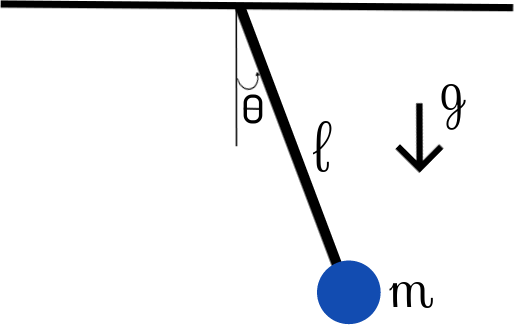
\includegraphics[scale=0.4]{problema5fig1}
 \caption{Péndulo simple.}
 \label{fig:problema5fig1}
\end{figure}

Recordemos que su lagrangiana es 

\begin{equation}
 L = \frac{1}{2}ml^2\dot{\theta}^2 + mgl\cos{\theta},
\end{equation}

el momento $p_\theta$ conjugado a $\theta$ es 

\begin{equation}
 p_\theta = \frac{\partial L}{\partial \dot{\theta}} = ml^2\dot{\theta},
\end{equation}

y por lo tanto la cantidad de Jacobi del sistema es 

\begin{equation}
 H = p_\theta \dot{\theta} - L = \frac{1}{2}ml^2\dot{\theta}^2 - mgl\cos{\theta},
\end{equation}

ahora para escribir la hamiltoniana del sistema escribimos la cantidad de Jacobi 
en términos de $\theta$ y $p_\theta$, 

\begin{equation}
 H = \frac{p_\theta^2}{2ml^2} - mgl\cos{\theta}.
\end{equation}

Ahora debido a que la energía cinética es una función cuadrática de las velocidades 
y la hamiltoniana no depende explícitamente del tiempo, entonces la hamiltoniana es 
la energía total del sistema, y aparte una integral de movimiento. Las trayectorias 
del sistema en el espacio de fases $(\theta,p_\theta)$ están dadas entonces por 

\begin{equation}
 E = \frac{p_\theta^2}{2ml^2} - mgl\cos{\theta},
 \label{eq:energiaTotalPendulo}
\end{equation}

donde $E$ es la energía total del sistema. Para analizar las trayectorias del sistema 
podemos despejar $p_\theta$ de \eqref{eq:energiaTotalPendulo}, 

\begin{equation}
 p_\theta = \sqrt{2ml^2(E - mgl\cos{\theta})},
\end{equation}

ahora si graficamos el espacio de fases para el péndulo simple podemos ver la 
forma de las trayectorias 

\begin{figure}[H]
 \center 
 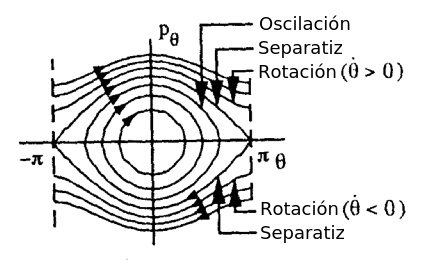
\includegraphics[scale=0.6]{problema5fig2}
 \caption{Trayectorias en el espacio de fases del péndulo simple}
 \label{fig:problema5fig2}
\end{figure}

Debemos notar que en la figura de arriba $\theta = \pi$ y  $\theta = -\pi$ son el 
mismo punto, debido a que el espacio de fases del péndulo simple es un cilindro, 
así que en realidad deberíamos imaginarnos al mismo como la figura de abajo 

\begin{figure}[H]
 \center 
 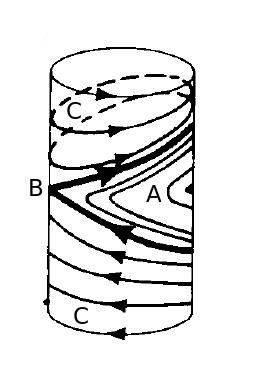
\includegraphics[scale=0.5]{problema5fig3}
 \caption{Trayectorias en el espacio de fases del péndulo simple. $A$ es la sección 
 de oscilación, $B$ es la separatriz y $C$ es la sección de rotación.}
 \label{fig:problema5fig3}
\end{figure}

Vemos entonces que tenemos entre $-mgl < E < mgl$ oscilación, la separatriz está 
en $E = mgl$ y tenemos rotación cuando $E > mgl$. En términos del enunciado y siguiendo 
a Arnold \cite{arnold}, en las secciones acotadas $A$ de la figura \ref{fig:problema5fig3} 
las trayectorias cerradas representan oscilaciones del péndulos y en las partes 
no acotadas, $C$ de la figura \ref{fig:problema5fig3} representan rotaciones del 
péndulo. 

\vspace{.3cm}

El tratamiento que haremos para llegar a las coordenadas solicitadas será el de 
la teoría de coordenadas de ángulo y acción. Según \cite{arnold} y \cite{calkin} 
se pueden construir estas coordenadas de ángulo y acción, que son a su vez coordenadas 
canónicas, en estas regiones, pero las coordenadas representarán cosas distintas y 
su forma diferirá dependiendo de la región que se esté tratando. Con esto podemos 
responder a las dos preguntas finales. Primero debemos resaltar que las coordenadas 
de acción y ángulo que construiremos, se dará el caso que encontraremos una integral 
de movimiento para cada región acotada, por lo tanto sí se pueden construir estas coordenadas 
en las regiones acotadas, pero como veremos su forma no será la misma para todas las 
regiones, por lo tanto la respuesta a que si se puede hacer de forma global menos 
algunos puntos o líneas, es en parte sí, si no consideramos los puntos hiperbólicos 
de las separatrices, pero no por la otra debido aunque podamos hallar estas coordenadas 
e integrales de movimiento para cada región acotada, su expresión no será exactamente 
la misma.

\vspace{.3cm}

Requerimos entonces una transformación canónica de coordenadas a unas coordenadas 
$(\phi,I)$ tales que 

\begin{equation}
 \frac{\partial H}{\partial \theta} = 0, \quad \dot{\phi} = \frac{\partial H}{\partial I} = 
 \omega (I) = \text{constante},
\end{equation}

es decir que $H$ sea una función solamente de $I$, y en cada región $\phi$ sea una 
coordenada ignorable, y por lo tanto $I$ sea una integral de movimiento, además 
la forma de $\phi$ será $\phi(t) = \omega(I)t + \phi(0)$. La variable $I$ se llama 
la coordenada canónica de acción y la variable $\phi$ se llama la coordenada canónica 
de ángulo. El tratamiento completo y común que se hace para las variables de 
acción y ángulo es con la teoría de Hamilton-Jacobi pero aunque utilizaremos algunos 
resultados que se obtienen de la misma, haremos el problema enmarcados en la teoría 
de Hamilton. Ya que las variables de acción y ángulo son canónicas, por hipótesis, sabemos 
que las transformaciones canónicas preservan el área en el espacio de fases, entonces 
podemos calcular la variable de acción con 

\begin{equation}
 I = \frac{1}{2\pi}\oint p_\theta d\theta = 
 \frac{1}{2\pi}\oint \sqrt{2ml^2(E - mgl\cos{\theta})} d\theta,
\end{equation}

que debemos evaluar en un ciclo cerrado entre $\theta_{min}$ y $\theta_{max}$, pero 
como el coseno es una función par, podemos escribir esta ecuación como 

\begin{equation}
 I = \frac{2}{\pi}\int_0^{\theta_{max}}  \sqrt{2ml^2(E - mgl\cos{\theta})} d\theta.
\end{equation}

Las soluciones a esta ecuación son funciones elípticas, tanto adentro como afuera de 
la separatriz. Y tenemos que 

\begin{itemize}
 \item En la separatriz $\theta_{max} = \pi$ y $E = mgl$.
 \item Adentro de la separatriz $\theta_{max} < \pi$ y $E < mgl$.
 \item Afuera de la separatriz $\theta_{max} > \pi$ y $E > mgl$.
\end{itemize}

Usando las funciones elípticas de primer tipo

\begin{equation}
 F\left(\frac{\pi}{2};k\right) = \int_0^{\frac{\pi}{2}} \frac{d\xi}{\sqrt{1 - k^2\sin{\xi}}} 
 = \int_0^1 \frac{dv}{(1-v^2)(1-k^2v^2)},
\end{equation}

donde $v=\sen{\xi}$ de manera que $dv = \cos{\xi}d\xi$, y las de segundo tipo 

\begin{equation}
 G\left(\frac{\pi}{2};k\right) = \int_0^{\frac{\pi}{2}} \sqrt{1 - k^2\sin{\xi}}d\xi = 
 \int_0^1 \frac{\sqrt{1 - k^2v^2}}{\sqrt{1 - v^2}}dv
\end{equation}

podemos escribir la variable de acción como

\begin{equation}
 I = \frac{8mglk}{\pi}G\left(\frac{\pi}{2};k\right) \quad \text{\textbf{Afuera de la 
 separatriz}}
\end{equation}

donde, $k = \frac{E + m^2g^2l^2}{2 m^2g^2l^2}$, y 

\begin{equation}
 I = \frac{8mgl}{\pi}\left(G\left(\frac{\pi}{2};k\right) - (1 - k^2)F\left(\frac{\pi}{2};k\right)\right) 
 \quad \text{\textbf{Adentro de la separatriz}}
\end{equation}

Estas $I$ serán integrales de movimiento en las regiones acotadas del espacio de fase. 
La frecuencia $\omega(I) = \frac{\partial H}{\partial I}$, será 

\begin{equation}
 \omega(I) = \frac{\pi mgl}{2F\left(\frac{\pi}{2};k\right)} \quad \text{Adentro de la 
 separatriz}
\end{equation}

y 

\begin{equation}
 \omega(I) = \frac{\pi mgl}{2F\left(\frac{\pi}{2};\frac{1}{k}\right)} \quad \text{Afuera de la 
 separatriz}
\end{equation}

Si ahora hacemos uso de $u = F(\xi;k)$ entonces $sn(u,k) = \sen{\xi} = \sen{\frac{\frac{\theta}{2}}{k}}$, 
podemos ahora escribir el impulso $p_\theta(\phi,I)$ en términos de estas nuevas variables 
como 

\begin{equation}
 p_\theta = 2mgl \sqrt{k^2 - k^2sn\left(\frac{2F(\xi;k)\phi}{\pi},k \right)},
\end{equation}

y con estas fórmulas podemos escribir entonces las transformaciones que buscabamos 

\begin{equation}
 \phi(t) = \omega(I)(t-t_0) \quad \text{y} \quad I(t) = \text{constante},
\end{equation}

donde 

\begin{equation}
 \omega(I) = \frac{\pi mgl}{2F(\xi;k)},
\end{equation}

y donde los valores de $I$ y $\omega(I)$ dependen de la región que se esté estudiando 
del péndulo, y hemos logrado lo solicitado que es encontrar una coordenada ignorable 
para cada región acotada, una integral de movimiento, y por ser construcciones de variables 
de acción y ángulo, la transformación a estas coordenadas es canónica.









\section{Problema 6}

Al hacer una transformación de punto dependiente del tiempo la hamiltoniana 
debe cambiarse por medio de 

$$
H' = H + \sum_j p_j \frac{\partial q^j}{\partial t},
$$

ver fórmula (189) de las notas.

\vspace{.3cm}

Al aplicar una transformación canónica de coordenadas dependiente del tiempo la 
hamiltoniana debe cambiar por 

$$
H' = H + \frac{\partial F}{\partial t}
$$

donde $F$ es la función generadora de la transformación. 

\vspace{.3cm}

Encuentre la relación entre estos dos resultados. Así mimos encuentre la relación 
entre la fórmula para la integral de movimiento ante una simetría que se vio en el 
contexto de la formulación lagrangiana y los generadores infinitesimales del grupo 
de dicha simetría.

\vspace{.3cm}

\underline{Solución:} \vspace{.3cm}

Recordemos un poco de donde salen estas ecuaciones. La primera,

\begin{equation} 
H' = H + \sum_j p_j \frac{\partial q^j}{\partial t},
\label{eq:hamiltonianaPunto}
\end{equation}

surge de una transformación de punto, definidas como aquella en la cual se propone 
un cambio de coordenadas de la variedad de configuración, i.e. 

\begin{equation}
 Q^i = Q^i(q,t),
\end{equation}

y los impulsos se generan utilizando la definición 

\begin{equation}
P_i = \frac{\partial L}{\partial \dot{Q}^i}.
\end{equation}

Veíamos que este tipo de transformaciones de coordenadas son canónicas, es decir, 
que hacen que las ecuaciones de movimiento conserven la forma hamiltoniana, pero 
la función hamiltoniana debe modificarse de acuerdo a \eqref{eq:hamiltonianaPunto}. 
Por otra parte, vimos que al aplicar una transformación canónica de coordenadas dependiente 
del tiempo, también se mantendrá la forma hamiltoniana de las ecuaciones ya que por 
definición esto es lo que hacen las transformaciones canónicas, y también en este 
caso debíamos cambiar la función hamiltoniana para que se mantuviera esto de acuerdo 
a 

\begin{equation}
 H' = H + \frac{\partial F}{\partial t}.
 \label{eq:hamiltonianaTiempo}
\end{equation}

Podemos entonces ahora ver que las transformaciones de punto como las hemos planteado 
son solo un ejemplo de las transformaciones canónicas de coordenadas dependientes 
del tiempo. Veamos ahora como están relacionadas estas dos ecuaciones. Para ver esto, 
supongamos que las $H'$ de \eqref{eq:hamiltonianaPunto} y \eqref{eq:hamiltonianaTiempo} 
son iguales, lo cual es plausible ya que ambas dejan invariantes a las ecuaciones 
de Hamilton y a la forma simpléctica, y pensemos que tenemos ambas ecuaciones 
y queremos ver entonces que relación tiene la $F$ con el segundo término de la 
derecha de la ecuación \eqref{eq:hamiltonianaPunto}, que son las que sobreviven 
al hacer la igualdad, es decir que tenemos 

\begin{equation}
 \sum_j p_j \frac{\partial q^j}{\partial t} = \frac{\partial F}{\partial t}.
\end{equation}

Sino queda claro lo que hacemos, sencillamente estamos viendo qué función generadora 
produce las transformaciones de punto, la cual vimos que era una transformación de 
coordenadas canónica. Debido a la expresión que tenemos para $P_i$ vemos también que 

\begin{equation}
 p_i = \sum_j P_j \frac{\partial Q^j}{\partial q^i},
\end{equation}

por lo tanto 

\begin{equation}
 \sum_j p_j \frac{\partial q^j}{\partial t} = 
 \sum_{ji} P_i\frac{\partial Q^i}{\partial q^j}\frac{\partial q^j}{\partial t} = 
 \sum_i P_i \frac{\partial Q^i}{\partial t}
\end{equation}

por lo tanto 

\begin{equation}
 \sum_i P_i \frac{\partial Q^i}{\partial t} = \frac{\partial F}{\partial t},
\end{equation}

pero debido a que $P_i$ no  depende del tiempo, vemos que 

\begin{equation}
 F = \sum_i P_i Q^i,
\end{equation}

es decir que la función generadora de una transformación de punto es una función 
generadora de segundo tipo $F_2 = F(q,P,t)$, por lo tanto podemos escribir 

\begin{equation}
 \boxed{F(q^i,P_i,t) = \sum_i P_i Q^i(q^i,t).}
\end{equation}

La cual entonces sería la función generadora de una transformación de punto.

\vspace{.3cm}

Ahora para ver la relación entre la fórmula para la integral de movimiento ante una
simetría que se vio en el contexto de la formulación lagrangiana y los generadores 
infinitesimales del grupo de dicha simetría, lo que haremos es hacer ver que 
la integral de movimiento, que era la energía total del sistema\footnote{En realidad 
la cantidad conservada era el inverso de la cantidad de Jacobi, pero asumiendo 
que la energía cinética es una función cuadrática de las velocidades y que 
la lagrangiana no depende explícitamente del tiempo esta es igual a la Hamiltoniana 
y a su vez a la energía total del sistema.}, se transforma con una transformación de 
punto con la misma función generadora que acabamos de encontrar, y que los generadores 
infinitesimales son los que nos permiten ver esto. Para hacer esto asumamos que 
el parámetro del grupo es $t$, entonces podemos expresar la integral de movimiento 
como

\begin{equation}
 E = \sum_i p_i\dot{q}^i - L = \sum_i \frac{\partial L}{\partial \dot{q}^i}\dot{q}^i - L,
\end{equation}

haciendo ahora la transformación, que debe ser invertible, $q^i = q^i(Q,t)$,

\begin{equation}
 \dot{Q}^i = \sum_j \frac{\partial Q^i}{\partial q^j}\dot{q}^j + \frac{\partial Q^i}{\partial t},
\end{equation}

\begin{equation}
 \dot{q}^i = \sum_j \frac{\partial q^i}{\partial Q^j}\dot{Q}^j + \frac{\partial q^i}{\partial t},
\end{equation}

tenemos que, usando algunos resultados obtenidos anteriormente

\begin{align*}
 \overline{E} &= \sum_i \frac{\partial L}{\partial \dot{Q}^i}\dot{Q}^i - L \\
 &= \sum_j \sum_k \sum_i \left[p_j\frac{\partial q^j}{\partial Q^i}\left( 
 \frac{\partial Q^i}{\partial q^k}\dot{q}^k + \frac{\partial Q^i}{\partial t}\right)\right] - L \\
 &= \sum_j p_j\dot{q}^j - L + \sum_i P_i \frac{\partial Q^i}{\partial t}
\end{align*}

\begin{equation}
 \therefore \overline{E} = E + \sum_i P_i \frac{\partial Q^i}{\partial t}
\end{equation}

y vemos ahora que la integral de movimiento, la energía total que es igual a la hamiltoniana $H$ en el caso 
que estudiamos, se transforma con una transformación de punto con una función generadora 
de tipo 2, $F_2(q,P,t)$, y la relación que existe entre la integral de movimiento y 
los generadores infinitesimales del grupo de la simetría con lo que vimos anteriormente 
es que estos son las funciones generadoras de la transformación de punto de dicha 
simetría. 


% \begin{equation}
%  F = \sum_j \int p_j \frac{\partial q^j}{\partial t}dt,
% \end{equation}
% 
% pero 
% 
% \begin{equation}
%  \frac{d}{dt}(p_jq^j) = q^j\frac{\partial p_j}{\partial t} +
%  p_j\frac{\partial q^j}{\partial t},
% \end{equation}
% 
% entonces 
% 
% \begin{equation}
%  F = \sum_j \int \left(\frac{d}{dt}(p_j q^j) - q^j\frac{\partial p_j}{\partial t}\right)dt
% \end{equation}
% 
% \begin{equation}
%  \boxed{\therefore F = \sum_j \left[p_j q^j - \int q^j \frac{\partial p_j}{\partial t}dt\right]}.
% \end{equation}

\section{Problema 7}

Cuando la hamiltoniana no depende explícitamente del tiempo las fórmulas para el 
campo vectorial hamiltoniano $\gamma[\bullet,V_H] = dH$, en el espacio de fase, 
y $\Gamma[V_H,\bullet] = 0$ en el espacio de fase extendido, son equivalentes. 
Demuestre esto de manera global, esto es, sin utilizar coordenadas.

\vspace{.3cm}

\underline{Solución:} \vspace{.3cm}

Recordemos que en el espacio extendido a la invariante diferencial de Poincaré-Cartan 
se define como

\begin{equation}
 \Gamma = \gamma - dH \wedge dt,
 \label{eq:poincareCartan}
\end{equation}

y el campo hamiltoniano se expresa como 

\begin{equation}
 V_{He} = V_H + \frac{\partial}{\partial t},
 \label{eq:campoHamiltonianoExt}
\end{equation}

donde $V_H$ es el campo hamiltoniano en el espacio de fase normal. Consideremos ahora 
que aplicamos la dos forma $\Gamma$ a este campo hamiltoniano extendido y a un campo 
vectorial arbitrario $X$, y utilizando la ecuación \eqref{eq:poincareCartan} tenemos 

\begin{equation}
 \Gamma[V_{He},X] = \gamma[V_{He},X] - dH \wedge dt[V_{He},X] = 0,
 \label{eq:equivalencia}
\end{equation}

ahora analicemos el valor de $dH \wedge dt[V_{He},X]$, utilizando \eqref{eq:campoHamiltonianoExt}
y el hecho de que ni $V_H$ ni $X$ tienen dependencia temporal

\begin{align*}
  dH \wedge dt[V_{He},X] &= dH \wedge dt[V_H,X] + dH \wedge dt[\frac{\partial}{\partial t},X] \\
  &= \left|\begin{matrix}
       dH[V_H] & dH[X] \\
       \cancelto{0}{dt[V_H]} & \cancelto{0}{dt[X]}
      \end{matrix}
      \right| + 
      \left|\begin{matrix}
       dH[\frac{\partial}{\partial t}] & dH[X] \\
       dt[\frac{\partial}{\partial t}] & \cancelto{0}{dt[X]}
      \end{matrix}
      \right| \\
  &= \left|\begin{matrix}
       dH[\frac{\partial}{\partial t}] & dH[X] \\
       1 & 0
      \end{matrix}
      \right|
\end{align*}

\begin{equation}
 \therefore dH \wedge dt[V_{He},X] = - dH[X]
\end{equation}

Ahora consideremos la forma de $\gamma[V_{He},X]$, utilizando la ecuación \eqref{eq:campoHamiltonianoExt}, 
vemos que pero si la hamiltoniana no depende del tiempo entonces no existirá en el campo hamiltoniano el 
término $\frac{\partial}{\partial t}$, y por lo tanto si $H$ no depende 
del tiempo

\begin{equation}
 \gamma[V_{He},X] = \gamma[V_H,X],
\end{equation}

y

\begin{equation}
 \Gamma[V_{He},X] = \Gamma[V_H,X],
\end{equation}

y ahora regresando a \eqref{eq:equivalencia} vemos que 

\begin{equation}
 \Gamma[V_H,X] = \gamma[V_H,X] - dH \wedge dt[V_H,X] = 0
\end{equation}

\begin{equation}
 \Gamma[V_H,X] = \gamma[V_H,X] + dH = 0
\end{equation}

y utilizando los resultados que hemos obtenido y el hecho de que $X$ es un campo 
vectorial arbitrario y que $ \gamma[V_H,X] =  - \gamma[X,V_H]$ vemos que 

\begin{equation}
 \gamma[V_H,X] = - dH[X] \Rightarrow \gamma[X,V_H] = dH[X]
\end{equation}

es totalmente equivalente a $\Gamma[V_H,X] = 0$ si $H$ no depende del tiempo, por lo tanto 

\begin{equation}
 \Gamma[V_H,\bullet] = 0 \Leftrightarrow \gamma[\bullet,X] = dH,
\end{equation}

lo cual era lo que queríamos demostrar. 

\begin{thebibliography}{10}
 \bibitem{arnold}
V. Arnold, \emph{Mathematical Methods of Classical Mechanics}, 2da edición, Springer-Verlang, 
1989.
\bibitem{calkin}
M. Calkin, \emph{Lagrangian and Hamiltonian Mechanics}, World Scientific, 1996.
\end{thebibliography}


\end{document}